%\documentclass{article}
\documentclass[oneside,11pt]{book}
\usepackage[margin=0.5in]{geometry}

% Package includes

\usepackage{caption}
\usepackage{changepage}
\usepackage[style=iso]{datetime2}
\usepackage{enumitem}
\usepackage{graphicx}
\usepackage[a4paper,margin=20mm]{geometry}
\usepackage{float}
\usepackage[colorlinks,citecolor=Navy,linkcolor=Navy]{hyperref}
\usepackage{longtable}
\usepackage{textcomp}
\usepackage[svgnames]{xcolor}
\usepackage[nocolor]{drawstack}

\setlength{\parskip}{0.5\baselineskip}

\newlength{\deftabcolsep}
\setlength\deftabcolsep{\tabcolsep}

\newenvironment{compacttables}{\setlength\tabcolsep{2pt}}{\setlength\tabcolsep{\deftabcolsep}}

% include this to debug page layout:
% \usepackage{showframe}

\captionsetup[table]{labelformat=empty}
\graphicspath{ {./images/} }

% commands to format instruction and register names
\newcommand{\insn}[1]{\texttt{#1}}
\newcommand{\reg}[1]{\texttt{#1}}
\newcommand{\an}{\texttt{a\textit{n}}}

% some formatting helpers
\newcommand{\fixme}[1]{\textcolor{purple}{\textit{FIXME: #1}}}
\newcommand{\note}[1]{
    \begin{adjustwidth}{3cm}{}
    \begin{flushright}
    \textit{#1}
    \end{flushright}
    \vspace{\parskip}
    \end{adjustwidth}
}

% Similar to \cellpt command from drawstack package, but points
% to the next divider between cells. See drawstack.sty for the
% definition of \cellptr. This differs only in "\value{cellnb}-0.5"
% instead of "\value{cellnb}-1".
\newcommand{\cellptrdiv}[1]{
  \draw[<-,line width=0.7pt] (0,\value{cellnb}-0.5) +(2,\value{ptrnb}*0.1) -- +(2.5,\value{ptrnb}*0.45);
  \draw (2.5,\value{ptrnb}*0.5+\value{cellnb}-0.5) node[anchor=west] {#1};
  \addtocounter{ptrnb}{1}
}


\begin{document}
	
\chapter*{Xtensa Instruction Set Architecture}

\chapter{Xtensa Instruction Set Architecture}
\pagestyle{plain}
\phantomsection
\setlength{\parindent}{2em}
\setlength{\parskip}{1em}

\section{Overview of Xtensa}


   Xtensa is a post-RISC ISA i.e it derives most of its features from RISC but also incorporates 
certain features where CISC is advantageous. Xtensa has 24-bit instructions (few are even 16 bits!),
unlike the conventional 32-bit instructions, to have code compactness.

  \textbf{Registers:}

  PC = Program Counter

  AR = General purpose registers

  SAR = Shifts and the Shift Amount Register

  PC essentially holds the address which is going to be executed.

  AR is general purpose registers, there are 64 32-bit registers however only 16 of them are 
visible/accessible at a time. This is windowed register.

  SAR register holds the shift amount required for shift instructions (logical left, logical right). 
Xtensa does not provide single-instruction shifts in which the shift amount is in general register 
(ar) operand. The shift amount is in SAR register.
  Windowed Register:

  General purpose registers (GPR) are used to store data temporarily for CPU while performing various operations. These registers are blazing fast but are limited in number (8 ~ 32).

  Typically, the number of registers present in the register file are equal to the registers directly accessible by the core. The Xtensa core can only access 16 GPR, namely a0 - a15. So the register file contains 16 registers.

  Xtensa also has a Windowed register option, which when enabled, extends this register file to contain 64 registers. Essentially, the register frame (a0 - a15) acts as a window, through which only 16 registers are visible, that slides on this large register file having 64 registers. And hence the name: Windowed register.

  Which 16 registers are visible is controlled by the WindowBase register. WindowBase register indicates where the window starts in the register file. Also, the shifting/rotation of this window occurs in units of 4. That means, the window starts at (WindowBase x 4)th position in the register file

\section{Windowed Register}

\underline{General purpose registers} (GPR) are used to store data temporarily for CPU while performing various operations. These registers are blazing fast but are limited in number (8 ~ 32).

Typically, the number of registers present in the register file are equal to the registers directly accessible by the core. The Xtensa core can only access 16 GPR, namely a0 - a15. So the register file contains 16 registers.

Xtensa also has a Windowed register option, which when enabled, extends this register file to contain 64 registers. Essentially, the register frame (a0 - a15) acts as a window, through which only 16 registers are visible, that slides on this large register file having 64 registers. And hence the name: Windowed register.

Which 16 registers are visible is controlled by the WindowBase register. WindowBase register indicates where the window starts in the register file. Also, the shifting/rotation of this window occurs in units of 4. That means, the window starts at (WindowBase x 4)$^{th}$ position in the register file

Windowed register


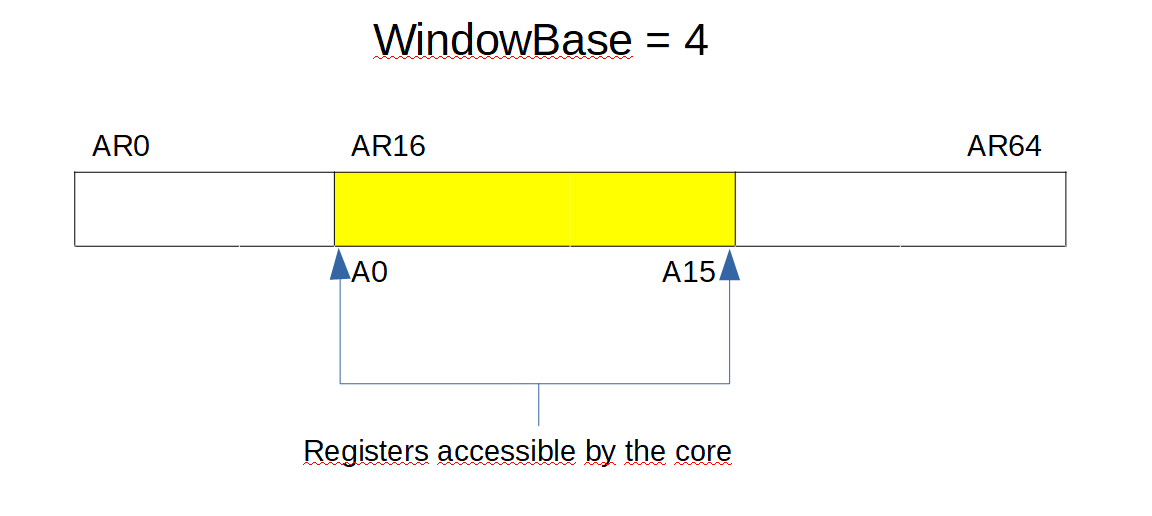
\includegraphics[scale=0.5]{Windowed_register.png}

Fig 1. Register window

\section*{Calling convention:}

 Xtensa supports two different application binary interfaces (ABI) which also includes the calling conventions.
 
1. Windowed register ABI

2. Call0 ABI

We will cover only Windowed register ABI.

Windowed register calling convention:

Return address is stored in a0 and the stack pointer is store in a1

Arguments to the functions are passed in both, registers and memory (stack). The first six arguments are passed in the registers and remaining go on the stack.

As for return values, they are returned in registers beginning from a2 till a5. If there are more than 4 values to be returned, the caller passes a pointer which is then populated by callee with all the return values.


\begin{longtable}{|p{5cm}|p{5cm}|}
	\hline
	Register & Use \\
	\hline
	a0 & Return Address\\ \hline
	a1 & Stack Pointer\\ \hline
	a2-a7 & Incomig Arguments\\ \hline
\end{longtable}

In Xtensa, subroutine calls are initiated using CALLN and CALLXN instructions. N is the windowed register option that specifies the amount by which the register window needs to be rotated for the callee. N can take values from 0, 4, 8 and 12. (call0/callx0 does not follow windowed register convention so further explanation does not apply for N = 0)

What does “rotation of window for the callee” exactly mean ?

When a subroutine is called using callN/callxN, WindowBase register is incremented by (N/4), so the registers visible when inside callee, through the window, would be different from caller because the register frame (a0 - a15) would have moved.

In general, for a windowed register call callN/callxN

\tcbset{
	frame code={}
	center title,
	left=0pt,
	right=0pt,
	top=0pt,
	bottom=0pt,
	colback=gray!70,
	colframe=white,
	width=\dimexpr\textwidth\relax,
	enlarge left by=0mm,
	boxsep=5pt,
	arc=0pt,outer arc=0pt,
}

\begin{tcolorbox}
	\textsc{aN of caller will be a0 of callee \newline a(N+1) of caller will be a1 of callee and so on…}
\end{tcolorbox}

So the caller needs to put the first argument of the callee in a(N+2), second in a(N+3) and so on..

While returning from the callee function, WindowBase register is decremented by (N/4) to keep the caller function registers same.

Let’s take an example:

\begin{tcolorbox}
\textsc{    /*\newline}
\textsc{	* void func(a,b)\newline}
\textsc{	* \{\newline}
\textsc{		*     ...\newline}
\textsc{		*     foo = bar(x,y);\newline}
\textsc{		*     ...\newline}
\textsc{		* \}\newline}
\textsc{	*/	\newline}
\textsc{		func:\newline}
\textsc{		...\newline}
\textsc{		mov         a10, x    // a10 is bar’s a2\newline}
\textsc{		mov         a11, y    // a11 is bar’s a3\newline}
\textsc{		call8       bar	\newline}
\textsc{		mov         foo, a10  // a10 is bar’s a2 (return value)\newline}
\textsc{		...}
\end{tcolorbox}

 When a function calls another function, it does not have to store its own arguments somewhere else to accomodate the arguments for the callee since the arguments of the callee is at a different physical location. The callee function internally will still use a2 to access its first argument but as you can see, a2 of the caller is at a different physical location than a2 of callee. If there was no windowing and the number of physical registers would be exactly 16 then a2 of caller and callee would be same. Thus for each function call, the data in these registers would have to be stored at some other memory location (stack) before calling any function and restore again after returning.

Accessing any memory location, other than register, is very slow and as a result this saving/restoring will have a negative impact on performance. So using windowed register convention saves us the overhead of such stores/restores and also reduces the code size.

\section*{Stack Layout:}
As mentioned, the stack pointer resides in a1 register. This stack pointer always points to the bottom of the stack!

Usually, function prologue sets up the stack for a function.

In Xtensa, ENTRY instruction is the function prologue

ENTRY instruction primarily does two things:
1. Allocates the stack frame for the function and sets the stack pointer.
2. Moves/rotates the register window by n as specified in the calln/callxn instruction.

Stack layout is always better explained through an illustration
%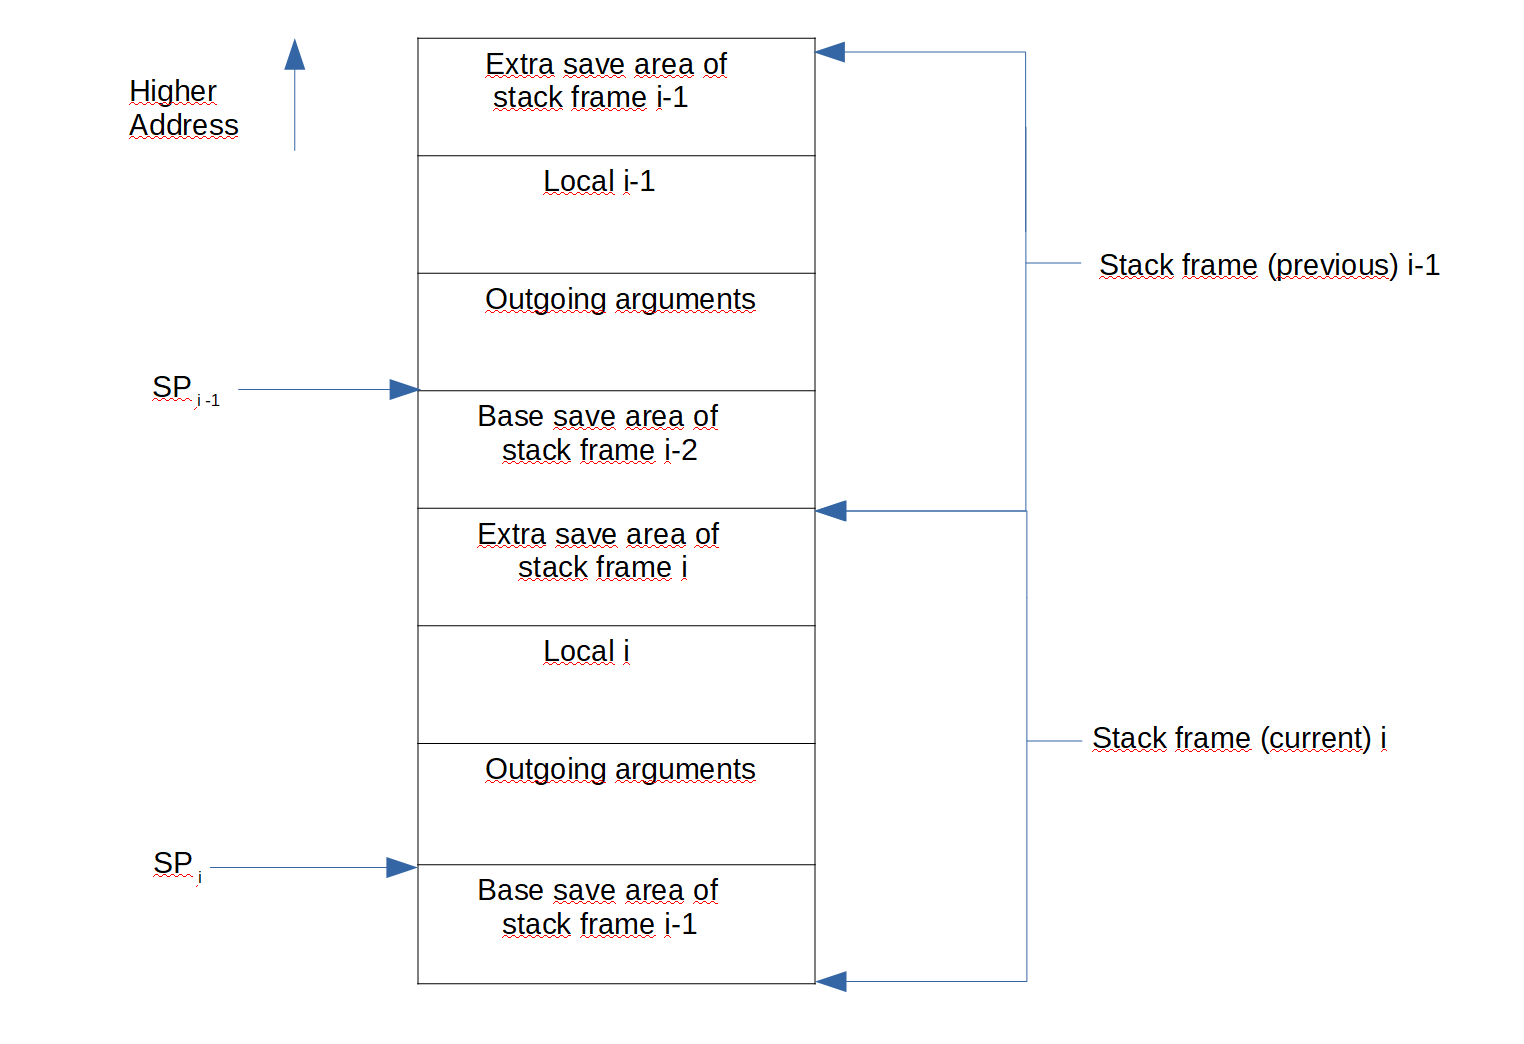
\includegraphics[scale=0.5]{Stack_layout.png}
\begin{figure}[h]
	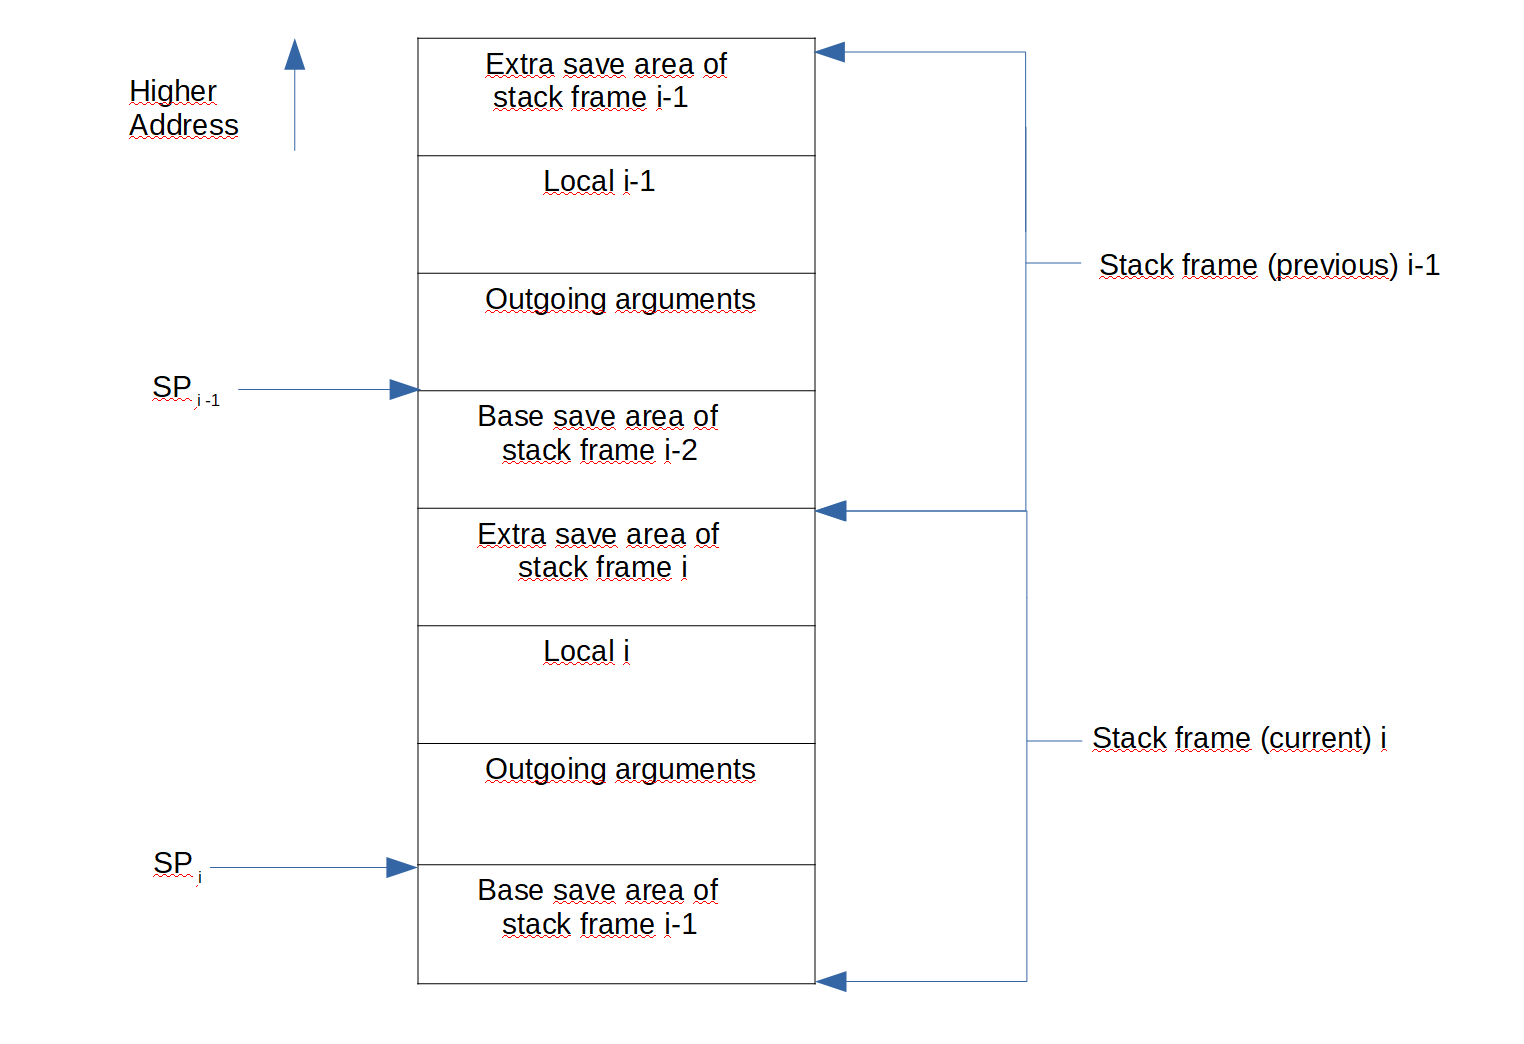
\includegraphics[width=12cm]{Stack_layout.png}
\end{figure}
Fig 2. Windowed ABI stack layout

For clarity, lets use sp as stack pointer instead of a1.

Like most architectures, in Xtensa too, stack grows downwards. If there are outgoing arguments, apart from the first 6 arguments, then they will go on the positive offset from sp. i.e 7th argument on sp, 8th on sp + 4 and so on. Above the outgoing arguments, local variables of that function are stored.

The region underneath the stack pointer, called Base Save Area, is of 16 bytes and reserved for saving the a0 - a3 of the caller (previous frame) when the window overflow exception occurs. If more registers of the caller are required to be saved then it is stored in the Extra Save Area at the top of the caller (previous) stack frame. The location of saving registers of the caller (i-1) frame is highlighed in the image.

With all the necessary points covered, let’s take an example and connect all the dots.

Suppose, each function call is carried out using call8 and we start with WindowBase = 4

Function A calls B, B calls C, C calls D… till I
i.e

\begin{tcolorbox}
\textsc{Functions:  A -> B -> C -> D -> E -> F -> G -> H -> I\newline}
\textsc{WindowBase: 4 -> 6 -> 8 -> 10 -> 12 -> 14 -> 0 -> 2 -> 4\newline}
\end{tcolorbox}

On each function call, the WindowBase will be incremented by 2 because call8 is used.

No. of bits in WindowBase register = $log_{2}$((No. of registers in register file)/4) = $log_{2}$(64⁄4) = 4. Thus the max value of WindowBase is 15.

As we have noticed, on the 9th function call the window wraps around to a point where the frame contains the data of a parent function, i.e a0,a1.. contains data of A. It implies that a8,a9.. of H are a0,a1.. of A.

A window overflow exception will be generated when H tries to modify a8,a9.. since it originally contains the context of A, so these must be saved to accommodate arguments of I. At this point, in the window overflow exception handler we must rotate the register window to frame A (WindowBase = 4).

a0 - a3 are stored in the Base Save Area of B’s stack frame. B’s stack frame is accessible since a9 is a1 of B, which is B’s stack pointer.
a4 - a7 are stored in the Extra Save Area of A’s stack frame.
Now whenever B returns, window underflow exception will be generated and we need to make sure that the corresponding exception handler would restore these values back into the registers.



\chapter*{Instruction Formats}

\chapter{Instruction Formats}

The contents of this chapter are derived from \cite{tensilica2008whitepaper,gcc,binutils,qemu}.

\phantomsection

\section {Instruction Fields}
\begin{description}[leftmargin=8em,style=nextline]
    \item[op0, op1, op2] 4-bit opcode fields
    \item[r, s, t] – 4-bit operand fields
\end{description}

\section {Functions}
\subsection{sign\_extend(imm)}

Extend an immediate to a 32-bit value by copying its left-most bit to all bits to the left.

\subsection{B4const(imm)}
\begin{verbatim}
int B4const(uint imm) {
    const int B4constValues[16] = {-1,1,2,3,4,5,6,7,8,10,12,16,32,64,128,256};
    return  B4constValues[imm];
}
\end{verbatim}

\subsection{B4constu(imm)}
\begin{verbatim}
uint B4constu(uint imm) {
    const int B4constuValues[16] = {32768,65536,2,3,4,5,6,7,8,10,12,16,32,64,128,256};
    return  B4constuValues[imm];
}
\end{verbatim}

\section {Assembler expressions}
\begin{description}[leftmargin=4em,style=nextline]
    \item[ar] – general purpose register correspondence to r operand field (AR[r])
    \item[as] – general purpose register correspondence to s operand field (AR[s])
    \item[at] – general purpose register correspondence to t operand field (AR[t])
    \item[sr] – special purpose register name
\end{description}

\section{Format descriptions}

\setlength{\tabcolsep}{8pt}
%\renewcommand{\arraystretch}{2}

%RRR format
\begin{table}[H]
    \caption{\textbf{RRR Instruction Format}}
    \begin{tabular}{llllllllllllllllllllllll}
       23 & & & 20 & 19 & & & 16 & 15 & & & 12 & 11 & & & 8 & 7 & & & 4 & 3 & & & 0 \\
        \hline
        \multicolumn{4}{|c|}{op2} & \multicolumn{4}{c|}{op1} & \multicolumn{4}{c|}{r} & \multicolumn{4}{c|}{s} & \multicolumn{4}{c|}{t} & \multicolumn{4}{c|}{$op0$}\\
        \hline
    \end{tabular}
\end{table}

%RRI4 format
\begin{table}[H]
    \caption{\textbf{RRI4 Instruction Format}}
    \begin{tabular}{llllllllllllllllllllllll}
        23 & & & 20 & 19 & & & 16 & 15 & & & 12 & 11 & & & 8 & 7 & & & 4 & 3 & & & 0 \\
        \hline
        \multicolumn{4}{|c|}{imm[3..0]} & \multicolumn{4}{c|}{op1} & \multicolumn{4}{c|}{r} & \multicolumn{4}{c|}{s} & \multicolumn{4}{c|}{t} & \multicolumn{4}{c|}{op0}\\
        \hline
    \end{tabular}
\end{table}

%RRI8 format
\begin{table}[H]
    \caption{\textbf{RRI8 Instruction Format}}
    \begin{tabular}{llllllllllllllllllllllll}
        23 & & & & & & & 16 & 15 & & & 12 & 11 & & & 8 & 7 & & & 4 & 3 & & & 0 \\
        \hline
        \multicolumn{8}{|c|}{imm[7..0]} & \multicolumn{4}{c|}{r} & \multicolumn{4}{c|}{s} & \multicolumn{4}{c|}{t} & \multicolumn{4}{c|}{op0}\\
        \hline
    \end{tabular}
\end{table}

%RI16 format
\begin{table}[H]
    \caption{\textbf{RI16 Instruction Format}}
    \begin{tabular}{llllllllllllllllllllllll}
        23 & & & & & & & & & & & & & & & 8 & 7 & & & 4 & 3 & & & 0 \\
        \hline
        \multicolumn{16}{|c|}{imm[15..0]} & \multicolumn{4}{c|}{t} & \multicolumn{4}{c|}{op0}\\
        \hline
    \end{tabular}
\end{table}

%RSR format
\begin{table}[H]
    \caption{\textbf{RSR Instruction Format}}
    \begin{tabular}{llllllllllllllllllllllll}
        23 & & & 20 & 19 & & & 16 & 15 & & & & & & & 8 & 7 & & & 4 & 3 & & & 0 \\
        \hline
        \multicolumn{4}{|c|}{imm[3..0]} & \multicolumn{4}{c|}{op1} &\multicolumn{8}{c|}{rs} & \multicolumn{4}{c|}{t} & \multicolumn{4}{c|}{op0}\\
        \hline
    \end{tabular}
\end{table}

%CALL format
\begin{table}[H]
    \caption{\textbf{CALL Instruction Format}}
    \begin{tabular}{llllllllllllllllllllllll}
        23 & & & & & & & & & & & & & & & & & 6 & 5 & 4 & 3 & & & 0 \\
        \hline
        \multicolumn{18}{|c|}{offset} & \multicolumn{2}{c|}{n} & \multicolumn{4}{c|}{op0}\\
        \hline
    \end{tabular}
\end{table}

%CALLX format
\begin{table}[H]
    \caption{\textbf{CALLX Instruction Format}}
    \begin{tabular}{llllllllllllllllllllllll}
        23 & & & 20 & 19 & & & 16 & 15 & & & 12 & 11 & & & 8 & 7 & 6 & 5 & 4 & 3 & & & 0 \\
        \hline
        \multicolumn{4}{|c|}{op2} & \multicolumn{4}{c|}{op1} & \multicolumn{4}{c|}{r} & \multicolumn{4}{c|}{s} & \multicolumn{2}{c|}{m} & \multicolumn{2}{c|}{n} & \multicolumn{4}{c|}{$op0$}\\
        \hline
    \end{tabular}
\end{table}

%BRI8 format
\begin{table}[H]
    \caption{\textbf{BRI8 Instruction Format}}
    \begin{tabular}{llllllllllllllllllllllll}
        23 & & & & & & & 16 & 15 & & & 12 & 11 & & & 8 & 7 & 6 & 5 & 4 & 3 & & & 0 \\
        \hline
        \multicolumn{8}{|c|}{imm[7..0]} & \multicolumn{4}{c|}{r} & \multicolumn{4}{c|}{s} & \multicolumn{2}{c|}{m} & \multicolumn{2}{c|}{n} & \multicolumn{4}{c|}{$op0$}\\
        \hline
    \end{tabular}
\end{table}

%BRI12 format
\begin{table}[H]
    \caption{\textbf{BRI12 Instruction Format}}
    \begin{tabular}{llllllllllllllllllllllll}
        23 & & & & & & & & & & & 12 & 11 & & & 8 & 7 & 6 & 5 & 4 & 3 & & & 0 \\
        \hline
        \multicolumn{12}{|c|}{imm[11..0]} & \multicolumn{4}{c|}{s} & \multicolumn{2}{c|}{m} & \multicolumn{2}{c|}{n} & \multicolumn{4}{c|}{$op0$}\\
        \hline
    \end{tabular}
\end{table}

%RRRN format
\begin{table}[H]
    \caption{\textbf{RRRN Instruction Format}}
    \begin{tabular}{llllllllllllllll}
        15 & & & 12 & 11 & & & 8 & 7 &  & & 4 & 3 & & & 0 \\
        \hline
        \multicolumn{4}{|c|}{r} & \multicolumn{4}{c|}{s} & \multicolumn{4}{c|}{t} & \multicolumn{4}{c|}{$op0$}\\
        \hline
    \end{tabular}
\end{table}

%RI7 format
\begin{table}[H]
    \caption{\textbf{RI7 Instruction Format}}
    \begin{tabular}{llllllllllllllll}
        15 & & & 12 & 11 & & & 8 & 7 & 6  & & 4 & 3 & & & 0 \\
        \hline
        \multicolumn{4}{|c|}{imm[3..0]} & \multicolumn{4}{c|}{s} & i & \multicolumn{3}{|c|}{imm[6..4]} & \multicolumn{4}{c|}{$op0$}\\
        \hline
    \end{tabular}
\end{table}

%RI6 format
\begin{table}[H]
    \caption{\textbf{RI6 Instruction Format}}
    \begin{tabular}{llllllllllllllll}
        15 & & & 12 & 11 & & & 8 & 7 & 6  & 5 & 4 & 3 & & & 0 \\
        \hline
        \multicolumn{4}{|c|}{imm[3..0]} & \multicolumn{4}{c|}{s} & i & \multicolumn{1}{c|}{z} & \multicolumn{2}{c|}{imm[5..4]} & \multicolumn{4}{c|}{$op0$}\\
        \hline
    \end{tabular}
\end{table}

\chapter*{Core Instruction Set}

\section*{Instructions encoded with RRR format}
%RRR format instructions
%\section{RRR format instructions}
\setlength{\tabcolsep}{4pt}
\renewcommand{\arraystretch}{2}
%\begin{table}[H]
	\begin{longtable}{llllllllllllllllllllllll  p{1cm}  p{6cm} | }
		\caption{Encoding\label{long}}\\
		23 & & & 20 & 19 & & & 16 & 15 & & & 12 & 11 & & & 8 & 7 & & & 4 & 3 & & & 0 & & \multicolumn{1}{c}{}\\
		\hline
        \endhead
		\multicolumn{4}{|c|}{0110} & \multicolumn{4}{c|}{0000} & \multicolumn{4}{c|}{r} & \multicolumn{4}{c|}{0001} & \multicolumn{4}{c|}{t} & \multicolumn{4}{c|}{0000} & \multicolumn{1}{c|}{$ABS$} & $If$ $AR[t]_{31}$ $then AR[r] \leftarrow -AR[t]$ \newline $else AR[r] \leftarrow AR[t]$ \newline endif \\ \hline
		\multicolumn{4}{|c|}{1000} & \multicolumn{4}{c|}{0000} & \multicolumn{4}{c|}{r} & \multicolumn{4}{c|}{s} & \multicolumn{4}{c|}{t} & \multicolumn{4}{c|}{0000} & \multicolumn{1}{c|}{$ADD$} & $AR[r] \leftarrow AR[s] + AR[t]$ \\ \hline
		\multicolumn{4}{|c|}{1001} & \multicolumn{4}{c|}{0000} & \multicolumn{4}{c|}{r} & \multicolumn{4}{c|}{s} & \multicolumn{4}{c|}{t} & \multicolumn{4}{c|}{0000} & \multicolumn{1}{c|}{$ADDX2$} & $AR[r] \leftarrow AR[s] + (AR[t]*2)$ \\ \hline
		\multicolumn{4}{|c|}{1010} & \multicolumn{4}{c|}{0000} & \multicolumn{4}{c|}{r} & \multicolumn{4}{c|}{s} & \multicolumn{4}{c|}{t} & \multicolumn{4}{c|}{0000} & \multicolumn{1}{c|}{$ADDX4$} & $AR[r] \leftarrow AR[s] + (AR[t]*4)$ \\ \hline
		\multicolumn{4}{|c|}{1011} & \multicolumn{4}{c|}{0000} & \multicolumn{4}{c|}{r} & \multicolumn{4}{c|}{s} & \multicolumn{4}{c|}{t} & \multicolumn{4}{c|}{0000} & \multicolumn{1}{c|}{$ADDX8$} & $AR[r] \leftarrow AR[s] + (AR[t]*8)$ \\ \hline
		\multicolumn{4}{|c|}{0001} & \multicolumn{4}{c|}{0000} & \multicolumn{4}{c|}{r} & \multicolumn{4}{c|}{s} & \multicolumn{4}{c|}{t} & \multicolumn{4}{c|}{0000} & \multicolumn{1}{c|}{$AND$} & $AR[r] \leftarrow AR[s] \& AR[t]$ \\ \hline
		\multicolumn{4}{|c|}{0000} & \multicolumn{4}{c|}{0000} & \multicolumn{4}{c|}{0010} & \multicolumn{4}{c|}{0000} & \multicolumn{4}{c|}{0011} & \multicolumn{4}{c|}{0000} & \multicolumn{1}{c|}{$DSYNC$} &  \\ \hline
		\multicolumn{4}{|c|}{0000} & \multicolumn{4}{c|}{0000} & \multicolumn{4}{c|}{0010} & \multicolumn{4}{c|}{0000} & \multicolumn{4}{c|}{0010} & \multicolumn{4}{c|}{0000} & \multicolumn{1}{c|}{$ESYNC$} &  \\ \hline
		\multicolumn{4}{|c|}{imm[3..0]} & \multicolumn{4}{c|}{010sh[4]} & \multicolumn{4}{c|}{r} & \multicolumn{4}{c|}{sh[3..0]} & \multicolumn{4}{c|}{t} & \multicolumn{4}{c|}{0000} & \multicolumn{1}{c|}{$EXTUI$} & $mi \leftarrow (0 || imm_{3..0}) + 1$ \newline $mask \leftarrow 0^{32-mi} || 1^{mi}$ \newline $AR[r] \leftarrow (0^{sh} || AR[s]_{31..sh}) AND mask$ \\ \hline
		\multicolumn{4}{|c|}{0000} & \multicolumn{4}{c|}{0000} & \multicolumn{4}{c|}{0010} & \multicolumn{4}{c|}{0000} & \multicolumn{4}{c|}{1101} & \multicolumn{4}{c|}{0000} & \multicolumn{1}{c|}{$EXTW$} &  \\ \hline	
		\multicolumn{4}{|c|}{0000} & \multicolumn{4}{c|}{0000} & \multicolumn{4}{c|}{0010} & \multicolumn{4}{c|}{0000} & \multicolumn{4}{c|}{0000} & \multicolumn{4}{c|}{0000} & \multicolumn{1}{c|}{$ISYNC$} &  \\ \hline
		\multicolumn{4}{|c|}{0000} & \multicolumn{4}{c|}{0000} & \multicolumn{4}{c|}{0010} & \multicolumn{4}{c|}{0000} & \multicolumn{4}{c|}{1100} & \multicolumn{4}{c|}{0000} & \multicolumn{1}{c|}{$MEMW$} &  \\ \hline
		\multicolumn{4}{|c|}{1000} & \multicolumn{4}{c|}{0011} & \multicolumn{4}{c|}{r} & \multicolumn{4}{c|}{s} & \multicolumn{4}{c|}{t} & \multicolumn{4}{c|}{0000} & \multicolumn{1}{c|}{$MOVEQZ$} & $condition \leftarrow AR[t] = 0^{32}$ \newline $if$ $condition$  $then$ \newline $AR[r] \leftarrow AR[s]$ \newline endif \\ \hline
		\multicolumn{4}{|c|}{1011} & \multicolumn{4}{c|}{0011} & \multicolumn{4}{c|}{r} & \multicolumn{4}{c|}{s} & \multicolumn{4}{c|}{t} & \multicolumn{4}{c|}{0000} & \multicolumn{1}{c|}{$MOVGEZ$} & $condition \leftarrow AR[t] >= 0^{32}$ \newline $if$ $condition$  $then$ \newline $AR[r] \leftarrow AR[s]$ \newline endif \\ \hline
		\multicolumn{4}{|c|}{1010} & \multicolumn{4}{c|}{0011} & \multicolumn{4}{c|}{r} & \multicolumn{4}{c|}{s} & \multicolumn{4}{c|}{t} & \multicolumn{4}{c|}{0000} & \multicolumn{1}{c|}{$MOVLTZ$} & $condition \leftarrow AR[t] < 0^{32}$ \newline $if$ $condition$  $then$ \newline $AR[r] \leftarrow AR[s]$ \newline endif \\ \hline
		\multicolumn{4}{|c|}{0110} & \multicolumn{4}{c|}{0011} & \multicolumn{4}{c|}{r} & \multicolumn{4}{c|}{0000} & \multicolumn{4}{c|}{t} & \multicolumn{4}{c|}{0000} & \multicolumn{1}{c|}{$NEG$} & $AR[r] \leftarrow 0^{32}-AR[t]$ \\ \hline
		\multicolumn{4}{|c|}{0000} & \multicolumn{4}{c|}{0000} & \multicolumn{4}{c|}{0010} & \multicolumn{4}{c|}{0000} & \multicolumn{4}{c|}{1111} & \multicolumn{4}{c|}{0000} & \multicolumn{1}{c|}{$NOP$} &  No operation \\ \hline
        \multicolumn{4}{|c|}{0010} & \multicolumn{4}{c|}{0000} & \multicolumn{4}{c|}{r} & \multicolumn{4}{c|}{s} & \multicolumn{4}{c|}{t} & \multicolumn{4}{c|}{0000} & \multicolumn{1}{c|}{$OR$} & $AR[r] \leftarrow AR[s] OR AR[t]$ \\ \hline		\multicolumn{4}{|c|}{0000} & \multicolumn{4}{c|}{0000} & \multicolumn{4}{c|}{0010} & \multicolumn{4}{c|}{0000} & \multicolumn{4}{c|}{0001} & \multicolumn{4}{c|}{0000} & \multicolumn{1}{c|}{$RSYNC$} &  \\ \hline
        \multicolumn{4}{|c|}{1010} & \multicolumn{4}{c|}{0001} & \multicolumn{4}{c|}{r} & \multicolumn{4}{c|}{s} & \multicolumn{4}{c|}{0000} & \multicolumn{4}{c|}{0000} & \multicolumn{1}{c|}{$SLL$} & $sh \leftarrow SAR_{5..0}$ \newline $AR[r] \leftarrow AR[s]_{31..31-sh} || 0^{sh}$ \\ \hline
        \multicolumn{4}{|c|}{000sh[4]} & \multicolumn{4}{c|}{0001} & \multicolumn{4}{c|}{r} & \multicolumn{4}{c|}{s} & \multicolumn{4}{c|}{sh[3..0]} & \multicolumn{4}{c|}{0000} & \multicolumn{1}{c|}{$SLLI$} & $AR[r] \leftarrow AR[s]_{31..31-sh} || 0^{sh}$ \\ \hline
        \multicolumn{4}{|c|}{1011} & \multicolumn{4}{c|}{0001} & \multicolumn{4}{c|}{r} & \multicolumn{4}{c|}{0000} & \multicolumn{4}{c|}{t} & \multicolumn{4}{c|}{0000} & \multicolumn{1}{c|}{$SRA$} & $sh \leftarrow SAR_{5..0}$ \newline $AR[r] \leftarrow AR[t]_{31}^{sh} || AR[t]_{31..sh}$ \\ \hline
        \multicolumn{4}{|c|}{101sh[4]} & \multicolumn{4}{c|}{0001} & \multicolumn{4}{c|}{r} & \multicolumn{4}{c|}{sh[3..0]} & \multicolumn{4}{c|}{t} & \multicolumn{4}{c|}{0000} & \multicolumn{1}{c|}{$SRAI$} & $AR[r] \leftarrow AR[t]_{31}^{sh} || AR[t]_{31..sh}$ \\ \hline
        \multicolumn{4}{|c|}{1000} & \multicolumn{4}{c|}{0001} & \multicolumn{4}{c|}{r} & \multicolumn{4}{c|}{s} & \multicolumn{4}{c|}{t} & \multicolumn{4}{c|}{0000} & \multicolumn{1}{c|}{$SRC$} & $sh \leftarrow SAR_{5..0}$ \newline $AR[r] \leftarrow AR[s]_{31-sh..sh} || AR[t]_{31..31-sh}$ \\ \hline
        \multicolumn{4}{|c|}{0001} & \multicolumn{4}{c|}{0001} & \multicolumn{4}{c|}{r} & \multicolumn{4}{c|}{0000} & \multicolumn{4}{c|}{t} & \multicolumn{4}{c|}{0000} & \multicolumn{1}{c|}{$SRL$} & $sh \leftarrow SAR_{5..0}$ \newline $AR[r] \leftarrow 0^{sh} || AR[t]_{31..sh}$ \\ \hline        
        \multicolumn{4}{|c|}{0100} & \multicolumn{4}{c|}{0001} & \multicolumn{4}{c|}{r} & \multicolumn{4}{c|}{sh} & \multicolumn{4}{c|}{t} & \multicolumn{4}{c|}{0000} & \multicolumn{1}{c|}{$SRLI$} & $AR[r] \leftarrow 0^{sh} || AR[t]_{31..sh}$ \\ \hline
        \multicolumn{4}{|c|}{0100} & \multicolumn{4}{c|}{0000} & \multicolumn{4}{c|}{0010} & \multicolumn{4}{c|}{s} & \multicolumn{4}{c|}{0000} & \multicolumn{4}{c|}{0000} & \multicolumn{1}{c|}{$SSA8L$} & $sh \leftarrow AR[s]_{1..0} || 0^3$ \newline $SAR \leftarrow sh$ \\ \hline
        \multicolumn{4}{|c|}{0100} & \multicolumn{4}{c|}{0000} & \multicolumn{4}{c|}{0010} & \multicolumn{4}{c|}{s} & \multicolumn{4}{c|}{0000} & \multicolumn{4}{c|}{0000} & \multicolumn{1}{c|}{$SSA8L$} & $sh \leftarrow AR[s]_{1..0} || 0^3$ \newline $SAR \leftarrow sh$ \\ \hline
        \multicolumn{4}{|c|}{0100} & \multicolumn{4}{c|}{0000} & \multicolumn{4}{c|}{0100} & \multicolumn{4}{c|}{sh[3..0]} & \multicolumn{4}{c|}{000sh[4]} & \multicolumn{4}{c|}{0000} & \multicolumn{1}{c|}{$SSL$} & $SAR \leftarrow 0^{27} || sh_{4..0}$ \\ \hline
        \multicolumn{4}{|c|}{0100} & \multicolumn{4}{c|}{0000} & \multicolumn{4}{c|}{0001} & \multicolumn{4}{c|}{s} & \multicolumn{4}{c|}{0000} & \multicolumn{4}{c|}{0000} & \multicolumn{1}{c|}{$SSL$} & $sh \leftarrow 0 || AR[s]_{4..0}$ \newline $SAR \leftarrow 32 - sh$ \\ \hline
        \multicolumn{4}{|c|}{0100} & \multicolumn{4}{c|}{0000} & \multicolumn{4}{c|}{0000} & \multicolumn{4}{c|}{s} & \multicolumn{4}{c|}{0000} & \multicolumn{4}{c|}{0000} & \multicolumn{1}{c|}{$SSR$} & $sh \leftarrow 0 || AR[s]_{4..0}$ \newline $SAR \leftarrow sh$ \\ \hline
		\multicolumn{4}{|c|}{1100} & \multicolumn{4}{c|}{0000} & \multicolumn{4}{c|}{r} & \multicolumn{4}{c|}{s} & \multicolumn{4}{c|}{t} & \multicolumn{4}{c|}{0000} & \multicolumn{1}{c|}{$SUB$} & $AR[r] \leftarrow AR[s] - AR[t]$ \\ \hline        
		\multicolumn{4}{|c|}{1101} & \multicolumn{4}{c|}{0000} & \multicolumn{4}{c|}{r} & \multicolumn{4}{c|}{s} & \multicolumn{4}{c|}{t} & \multicolumn{4}{c|}{0000} & \multicolumn{1}{c|}{$SUBX2$} & $AR[r] \leftarrow AR[s] - (AR[t]*2)$ \\ \hline        
		\multicolumn{4}{|c|}{1110} & \multicolumn{4}{c|}{0000} & \multicolumn{4}{c|}{r} & \multicolumn{4}{c|}{s} & \multicolumn{4}{c|}{t} & \multicolumn{4}{c|}{0000} & \multicolumn{1}{c|}{$SUBX4$} & $AR[r] \leftarrow AR[s] - (AR[t]*4)$ \\ \hline        
		\multicolumn{4}{|c|}{1111} & \multicolumn{4}{c|}{0000} & \multicolumn{4}{c|}{r} & \multicolumn{4}{c|}{s} & \multicolumn{4}{c|}{t} & \multicolumn{4}{c|}{0000} & \multicolumn{1}{c|}{$SUBX8$} & $AR[r] \leftarrow AR[s] - (AR[t]*8)$ \\ \hline
		\multicolumn{4}{|c|}{0011} & \multicolumn{4}{c|}{0000} & \multicolumn{4}{c|}{r} & \multicolumn{4}{c|}{s} & \multicolumn{4}{c|}{t} & \multicolumn{4}{c|}{0000} & \multicolumn{1}{c|}{$XOR$} & $AR[r] \leftarrow AR[s] XOR AR[t]$ \\ \hline
		\multicolumn{4}{|c|}{0110} & \multicolumn{4}{c|}{0001} & \multicolumn{8}{c|}{sr} & \multicolumn{4}{c|}{t} & \multicolumn{4}{c|}{0000} & \multicolumn{1}{c|}{$XSR$} & $tmp \leftarrow AR[t]$ \newline $AR[t] \leftarrow SR[sr]$ \newline $SR[sr] \leftarrow tmp$ \\ \hline
	\end{longtable}
%\end{table}

%\begin{longtable}[H]
	\begin{longtable}{|p{5cm}|p{5cm}|}
		\caption{Assembler\label{long}}\\
		\hline
		Instruction & \\
		\hline
        \endhead
		ABS & abs ar, at\\ \hline
		ADD & add ar, as, at\\ \hline
		ADDX2 & addx2 ar, as, at\\ \hline
		ADDX4 & addx4 ar, as, at\\ \hline
		ADDX8 & addx8 ar, as, at\\ \hline
		AND & and ar, as, at\\ \hline
		DSYNC & dsync\\ \hline
		ESYNC & esync\\ \hline
		EXTUI & extui ar, as, sh\_imm, mask\_imm\\ \hline
		EXTW & extw\\ \hline
		ISYNC & isync\\ \hline
		MEMW & memw\\ \hline
		MOVEQZ & moveqz ar, as, at\\ \hline
		MOVGEZ & movgez ar, as, at\\ \hline
		MOVLTZ & movltz ar, as, at\\ \hline
		NEG & neg ar, as\\ \hline
		NOP & nop\\ \hline
		OR & or ar, as, at\\ \hline
		RSYNC & rsync\\ \hline
		SLL & sll ar, as\\ \hline
		SLLI & slli ar, as, sh\_imm\\ \hline
		SRA & sra ar, at\\ \hline
		SRAI & srai ar, at, sh\_imm\\ \hline
		SRC & src ar, as, at\\ \hline
		SRL & srl ar, as\\ \hline
		SRLI & srli ar, at, sh\_imm\\ \hline
		SSA8L & ssa8l as\\ \hline
		SSAI & ssai sh\_imm\\ \hline
		SSL & ssl as\\ \hline
		SSR & ssr as\\ \hline
		SUB & sub ar, as, at\\ \hline
        SUBX2 & subx2 ar, as, at\\ \hline
        SUBX4 & subx4 ar, as, at\\ \hline
        SUBX8 & subx8 ar, as, at\\ \hline
	\end{longtable}
% \end{longtable}
\section*{Instructions encoded with RRI8 format}
\section{Instructions encoded with RRI8 format}
\begin{smalltables}
	\begin{longtable}{llllllllllllllllllllllll  p{1cm}  p{7cm} | }
		\caption{Encoding\label{long}}\\
		23 & & & & & & & 16 & 15 & & & 12 & 11 & & & 8 & 7 & & & 4 & 3 & & & 0 & & \multicolumn{1}{c}{}\\
		\hline
        \endhead
		\multicolumn{8}{|c|}{imm[7..0]} & \multicolumn{4}{c|}{1100} & \multicolumn{4}{c|}{s} & \multicolumn{4}{c|}{t} & \multicolumn{4}{c|}{0010} & \multicolumn{1}{c|}{$ADDI$} & $AR[s] \leftarrow AR[t] + imm$ \\ \hline
		\multicolumn{8}{|c|}{imm[7..0]} & \multicolumn{4}{c|}{1101} & \multicolumn{4}{c|}{s} & \multicolumn{4}{c|}{t} & \multicolumn{4}{c|}{0010} & \multicolumn{1}{c|}{$ADDMI$} & $AR[s] \leftarrow AR[t] + (imm_7^{16} || imm_{7..0} || 0^8)$ \\ \hline
		\multicolumn{8}{|c|}{imm[7..0]} & \multicolumn{4}{c|}{0100} & \multicolumn{4}{c|}{s} & \multicolumn{4}{c|}{t} & \multicolumn{4}{c|}{0111} & \multicolumn{1}{c|}{$BALL$} & $offset \leftarrow sign\_extend(imm)$ \newline $condition \leftarrow AR[s] AND AR[t] = 0^{32}$ \newline if condition then \newline $PC \leftarrow PC + offset + 4$ \newline endif\\ \hline
		\multicolumn{8}{|c|}{imm[7..0]} & \multicolumn{4}{c|}{1000} & \multicolumn{4}{c|}{s} & \multicolumn{4}{c|}{t} & \multicolumn{4}{c|}{0111} & \multicolumn{1}{c|}{$BANY$} & $offset \leftarrow sign\_extend(imm)$ \newline  $condition \leftarrow$ (NOT AR[s]) AND AR[t] $\neq 0^{32}$ \newline if condition then \newline $PC \leftarrow PC + offset + 4$ \newline endif\\ \hline
		\multicolumn{8}{|c|}{imm[7..0]} & \multicolumn{4}{c|}{0101} & \multicolumn{4}{c|}{s} & \multicolumn{4}{c|}{t} & \multicolumn{4}{c|}{0111} & \multicolumn{1}{c|}{$BBC$} & $offset \leftarrow sign\_extend(imm)$ \newline $bit \leftarrow AR[t]_{4..0}$ \newline $condition \leftarrow$ $AR[s]_{bit} = 0$ \newline if condition then \newline $PC \leftarrow PC + offset + 4$ \newline endif\\ \hline
		\multicolumn{8}{|c|}{imm[7..0]} & \multicolumn{4}{c|}{011b[4]} & \multicolumn{4}{c|}{s} & \multicolumn{4}{c|}{b[3..0]} & \multicolumn{4}{c|}{0111} & \multicolumn{1}{c|}{$BBCI$} & $offset \leftarrow signe\_extend(imm)$ \newline $condition \leftarrow AR[s]_{b} = 0$ \newline if condition then \newline $PC \leftarrow PC + offset + 4$ \newline endif\\ \hline
		\multicolumn{8}{|c|}{imm[7..0]} & \multicolumn{4}{c|}{1101} & \multicolumn{4}{c|}{s} & \multicolumn{4}{c|}{t} & \multicolumn{4}{c|}{0111} & \multicolumn{1}{c|}{$BBS$} & $offset \leftarrow sign\_extend(imm)$ \newline $bit \leftarrow AR[t]_{4..0}$ \newline $condition \leftarrow$ $AR[s]_{bit} \neq 0$ \newline if condition then \newline $PC \leftarrow PC + offset + 4$ \newline endif\\ \hline
		\multicolumn{8}{|c|}{imm[7..0]} & \multicolumn{4}{c|}{111b[4]} & \multicolumn{4}{c|}{s} & \multicolumn{4}{c|}{b[3..0]} & \multicolumn{4}{c|}{0111} & \multicolumn{1}{c|}{$BBSI$} & $offset \leftarrow sign\_extend(imm)$ \newline $condition \leftarrow AR[s]_{b} \neq 0$ \newline if condition then \newline $PC \leftarrow PC + offset + 4$ \newline endif\\ \hline
%BEQ
		\multicolumn{8}{|c|}{imm[7..0]} & \multicolumn{4}{c|}{0001} & \multicolumn{4}{c|}{s} & \multicolumn{4}{c|}{t} & \multicolumn{4}{c|}{0111} & \multicolumn{1}{c|}{$BEQ$} & $offset \leftarrow sign\_extend(imm)$ \newline $condition \leftarrow (AR[t]=AR[s])$ \newline if condition then \newline $PC \leftarrow PC + offset + 4$ \newline endif\\ \hline
		\multicolumn{8}{|c|}{imm[7..0]} & \multicolumn{4}{c|}{r} & \multicolumn{4}{c|}{s} & \multicolumn{4}{c|}{0010} & \multicolumn{4}{c|}{0110} & \multicolumn{1}{c|}{$BEQI$} & $offset \leftarrow sign\_extend(imm)$ \newline $condition \leftarrow (AR[t] = B4Const[r])$ \newline if condition then \newline $PC \leftarrow PC + offset + 4$ \newline endif\\ \hline

		\multicolumn{8}{|c|}{imm[7..0]} & \multicolumn{4}{c|}{1010} & \multicolumn{4}{c|}{s} & \multicolumn{4}{c|}{t} & \multicolumn{4}{c|}{0111} & \multicolumn{1}{c|}{$BGE$} & $offset \leftarrow sign\_extend(imm)$ \newline $condition \leftarrow (AR[t] >= AR[s])$ \newline if condition then \newline $PC \leftarrow PC + offset + 4$ \newline endif\\ \hline
		\multicolumn{8}{|c|}{imm[7..0]} & \multicolumn{4}{c|}{r} & \multicolumn{4}{c|}{s} & \multicolumn{4}{c|}{1110} & \multicolumn{4}{c|}{0110} & \multicolumn{1}{c|}{$BGEI$} & $offset \leftarrow sign\_extend(imm)$ \newline $condition \leftarrow (AR[t] >= B4Const[r])$ \newline if condition then \newline $PC \leftarrow PC + offset + 4$ \newline endif\\ \hline
		\multicolumn{8}{|c|}{imm[7..0]} & \multicolumn{4}{c|}{1011} & \multicolumn{4}{c|}{s} & \multicolumn{4}{c|}{t} & \multicolumn{4}{c|}{0111} & \multicolumn{1}{c|}{$BGEU$} & $offset \leftarrow sign\_extend(imm)$ \newline $condition \leftarrow (0||AR[t]) >= (0||AR[s])$ \newline if condition then \newline $PC \leftarrow PC + offset + 4$ \newline endif\\ \hline
        \multicolumn{8}{|c|}{imm[7..0]} & \multicolumn{4}{c|}{r} & \multicolumn{4}{c|}{s} & \multicolumn{4}{c|}{1111} & \multicolumn{4}{c|}{0110} & \multicolumn{1}{c|}{$BGEUI$} & $offset \leftarrow sign\_extend(imm)$ \newline $condition \leftarrow (0||AR[t]) >= (0||B4Const[r])$ \newline if condition then \newline $PC \leftarrow PC + offset + 4$ \newline endif\\ \hline
		\multicolumn{8}{|c|}{imm[7..0]} & \multicolumn{4}{c|}{0010} & \multicolumn{4}{c|}{s} & \multicolumn{4}{c|}{t} & \multicolumn{4}{c|}{0111} & \multicolumn{1}{c|}{$BLT$} & $offset \leftarrow sign\_extend(imm)$ \newline $condition \leftarrow (AR[s] < AR[t])$ \newline if condition then \newline $PC \leftarrow PC + offset + 4$ \newline endif\\ \hline
        \multicolumn{8}{|c|}{imm[7..0]} & \multicolumn{4}{c|}{r} & \multicolumn{4}{c|}{s} & \multicolumn{4}{c|}{1010} & \multicolumn{4}{c|}{0110} & \multicolumn{1}{c|}{$BLTI$} & $offset \leftarrow sign\_extend(imm)$ \newline $condition \leftarrow (AR[t] < B4Const[r])$ \newline if     condition then \newline $PC \leftarrow PC + offset + 4$ \newline endif\\ \hline
		\multicolumn{8}{|c|}{imm[7..0]} & \multicolumn{4}{c|}{0011} & \multicolumn{4}{c|}{s} & \multicolumn{4}{c|}{t} & \multicolumn{4}{c|}{0111} & \multicolumn{1}{c|}{$BLTU$} & $offset \leftarrow sign\_extend(imm)$ \newline $condition \leftarrow (0||AR[t]) < (0||AR[s])$ \newline if condition then \newline $PC \leftarrow PC + offset + 4$ \newline endif\\ \hline
        \multicolumn{8}{|c|}{imm[7..0]} & \multicolumn{4}{c|}{r} & \multicolumn{4}{c|}{s} & \multicolumn{4}{c|}{1011} & \multicolumn{4}{c|}{0110} & \multicolumn{1}{c|}{$BLTUI$} & $offset \leftarrow sign\_extend(imm)$ \newline $condition \leftarrow (0||AR[t]) < (0||B4Const[r])$ \newline if condition then \newline $PC \leftarrow PC + offset + 4$ \newline endif\\ \hline
       \multicolumn{8}{|c|}{imm[7..0]} & \multicolumn{4}{c|}{1100} & \multicolumn{4}{c|}{s} & \multicolumn{4}{c|}{t} & \multicolumn{4}{c|}{0111} & \multicolumn{1}{c|}{$BNALL$} & $offset \leftarrow sign\_extend(imm)$ \newline $condition \leftarrow (AR[s]$ $AND$ $AR[t])$ $\neq0^{32}$ \newline if condition then \newline $PC \leftarrow PC + offset + 4$ \newline endif\\ \hline
%BNE
	   \multicolumn{8}{|c|}{imm[7..0]} & \multicolumn{4}{c|}{1001} & \multicolumn{4}{c|}{s} & \multicolumn{4}{c|}{t} & \multicolumn{4}{c|}{0111} & \multicolumn{1}{c|}{$BNE$} & $offset \leftarrow sign\_extend(imm)$ \newline $condition \leftarrow (AR[t] \neq AR[s])$ \newline if condition then \newline $PC \leftarrow PC + offset + 4$ \newline endif\\ \hline
       \multicolumn{8}{|c|}{imm[7..0]} & \multicolumn{4}{c|}{r} & \multicolumn{4}{c|}{s} & \multicolumn{4}{c|}{0110} & \multicolumn{4}{c|}{0110} & \multicolumn{1}{c|}{$BNEI$} & $offset \leftarrow sign\_extend(imm)$ \newline $condition \leftarrow (AR[t] \neq B4Const[r])$ \newline if condition then \newline $PC \leftarrow PC + offset + 4$ \newline endif\\ \hline
       \multicolumn{8}{|c|}{imm[7..0]} & \multicolumn{4}{c|}{0000} & \multicolumn{4}{c|}{s} & \multicolumn{4}{c|}{t} & \multicolumn{4}{c|}{0111} & \multicolumn{1}{c|}{$BNONE$} & $offset \leftarrow sign\_extend(imm)$ \newline $condition \leftarrow (AR[s]$ $AND$ $AR[t])$ $=$ $0^{32}$ \newline if condition then \newline $PC \leftarrow PC + offset + 4$ \newline endif\\ \hline
%L8UI
	   \multicolumn{8}{|c|}{imm[7..0]} & \multicolumn{4}{c|}{0000} & \multicolumn{4}{c|}{s} & \multicolumn{4}{c|}{t} & \multicolumn{4}{c|}{0010} & \multicolumn{1}{c|}{$L8UI$} & $offset \leftarrow sign\_extend(imm)$ \newline $vAddr \leftarrow AR[s] + offset$ \newline $mem \leftarrow LoadMemory(vAddr, 8)$ \newline $AR[t] \leftarrow 0^{24}||mem_{7..0}$\\ \hline
	   \multicolumn{8}{|c|}{imm[7..0]} & \multicolumn{4}{c|}{1001} & \multicolumn{4}{c|}{s} & \multicolumn{4}{c|}{t} & \multicolumn{4}{c|}{0010} & \multicolumn{1}{c|}{$L16SI$} & $offset \leftarrow sign\_extend(imm)$ \newline $vAddr \leftarrow AR[s] + offset$ \newline $mem \leftarrow LoadMemory(vAddr, 16)$ \newline $AR[t] \leftarrow mem_{15}^{16}||mem_{15..0}$\\ \hline
	   \multicolumn{8}{|c|}{imm[7..0]} & \multicolumn{4}{c|}{0001} & \multicolumn{4}{c|}{s} & \multicolumn{4}{c|}{t} & \multicolumn{4}{c|}{0010} & \multicolumn{1}{c|}{$L16UI$} & $offset \leftarrow sign\_extend(imm)$ \newline $vAddr \leftarrow AR[s] + offset$ \newline $mem \leftarrow LoadMemory(vAddr, 16)$ \newline $AR[t] \leftarrow 0^{16}||mem_{15..0}$\\ \hline
	   \multicolumn{8}{|c|}{imm[7..0]} & \multicolumn{4}{c|}{0010} & \multicolumn{4}{c|}{s} & \multicolumn{4}{c|}{t} & \multicolumn{4}{c|}{0010} & \multicolumn{1}{c|}{$L32I$} & $offset \leftarrow sign\_extend(imm)$ \newline $vAddr \leftarrow AR[s] + offset$ \newline $mem \leftarrow LoadMemory(vAddr, 32)$ \newline $AR[t] \leftarrow mem_{31..0}$\\ \hline
	   \multicolumn{8}{|c|}{imm[7..0]} & \multicolumn{4}{c|}{1010} & \multicolumn{4}{c|}{imm[11..8]} & \multicolumn{4}{c|}{t} & \multicolumn{4}{c|}{0010} & \multicolumn{1}{c|}{$MOVI$} & $AR[s] \leftarrow sign\_extend(imm)$ \\ \hline
%S8I
       \multicolumn{8}{|c|}{imm[7..0]} & \multicolumn{4}{c|}{0100} & \multicolumn{4}{c|}{s} & \multicolumn{4}{c|}{t} & \multicolumn{4}{c|}{0010} & \multicolumn{1}{c|}{$S8I$} & $offset \leftarrow sign\_extend(imm)$ \newline $vAddr \leftarrow AR[s] + offset$ \newline $StoreMemory(vAddr, 8, AR[t]_{7..0})$\\ \hline
       \multicolumn{8}{|c|}{imm[7..0]} & \multicolumn{4}{c|}{0101} & \multicolumn{4}{c|}{s} & \multicolumn{4}{c|}{t} & \multicolumn{4}{c|}{0010} & \multicolumn{1}{c|}{$S16I$} & $offset \leftarrow sign\_extend(imm)$ \newline $vAddr \leftarrow AR[s] + offset$ \newline $StoreMemory(vAddr, 16, AR[t]_{15..0})$\\ \hline
       \multicolumn{8}{|c|}{imm[7..0]} & \multicolumn{4}{c|}{0110} & \multicolumn{4}{c|}{s} & \multicolumn{4}{c|}{t} & \multicolumn{4}{c|}{0010} & \multicolumn{1}{c|}{$S32I$} & $offset \leftarrow sign\_extend(imm)$ \newline $vAddr \leftarrow AR[s] + offset$ \newline $StoreMemory(vAddr, 32, AR[t]_{31..0})$\\ \hline
	\end{longtable}

	\begin{longtable}{|p{5cm}|p{5cm}|}
		\caption{Assembler\label{long}}\\
		\hline
		Instruction & \\
		\hline
		ADDI & addi at, as, imm\\ \hline
		ADDMI & addmi at, as, imm\\ \hline
		BALL & ball as, at, target\\ \hline
		BANY & bany as, at, target\\ \hline
		BBC & bbc as, at, target\\ \hline
		BBCI & bbci as, imm, target\\ \hline
		BBS & bbs as, at, target\\ \hline
		BBSI & bbsi as, imm, target\\ \hline
		BEQ & beq as, at, target\\ \hline
		BEQI & beqi as, imm, target\\ \hline
		BGE & bge as, at, target\\ \hline
		BGEI & bgei as, imm, target\\ \hline
		BGEU & bgeu as, at, target\\ \hline
		BGEUI & bgeui as, imm, target\\ \hline
		BLT & blt as, at, target\\ \hline
		BLTI & blti as, imm, target\\ \hline
		BLTU & bltu as, at, target\\ \hline
		BLTUI & bltui as, imm, target\\ \hline
		BNALL & bnall as, at, target\\ \hline
		BNE & bne as, at, target\\ \hline
		BNEI & bnei as, imm, target\\ \hline
		BNONE & bnone as, at, target\\ \hline
		L8UI & l8ui at, as, imm\\ \hline
		L16SI & l16si at, as, imm\\ \hline
		L16UI & l16ui at, as, imm\\ \hline
		L32I & l32i at, as, imm\\ \hline
		MOVI & movi at, imm\\ \hline
		S8I & s8i at, as, imm\\ \hline
		S16I & s16i at, as, imm\\ \hline
		S32I & s32i at, as, imm\\ \hline
	\end{longtable}
\end{smalltables}
\section*{Instructions encoded with BRI12 format}
\section{Instructions encoded with BRI12 format}
%\begin{table}[H]
	\begin{longtable}{llllllllllllllllllllllll  p{1cm}  p{7cm} | }
		\caption{Encoding\label{long}}\\
		23 & & & & & & & & & & & 12 & 11 & & & 8 & 7 & & & 4 & 3 & & & 0 & &
		\multicolumn{1}{c}{}\\
		\hline
		%BEQZ
		\multicolumn{12}{|c|}{imm[11..0]} & \multicolumn{4}{c|}{s} & \multicolumn{4}{c|}{0001} & \multicolumn{4}{c|}{0110} & \multicolumn{1}{c|}{$BEQZ$} & $offset \leftarrow sign\_extend(imm)$ \newline $condition \leftarrow (AR[s] = 0^{32})$ \newline if condition then \newline $PC \leftarrow PC + offset + 4$ \newline endif\\ \hline
		\multicolumn{12}{|c|}{imm[11..0]} & \multicolumn{4}{c|}{s} & \multicolumn{4}{c|}{1101} & \multicolumn{4}{c|}{0110} & \multicolumn{1}{c|}{$BGEZ$} & $offset \leftarrow sign\_extend(imm)$ \newline $condition \leftarrow (AR[s] >= 0^{32})$ \newline if condition then \newline $PC \leftarrow PC + offset + 4$ \newline endif\\ \hline
		\multicolumn{12}{|c|}{imm[11..0]} & \multicolumn{4}{c|}{s} & \multicolumn{4}{c|}{1001} & \multicolumn{4}{c|}{0110} & \multicolumn{1}{c|}{$BLTZ$} & $offset \leftarrow sign\_extend(imm)$ \newline $condition \leftarrow (AR[s] < 0^{32})$ \newline if condition then \newline $PC \leftarrow PC + offset + 4$ \newline endif\\ \hline
		\multicolumn{12}{|c|}{imm[11..0]} & \multicolumn{4}{c|}{s} & \multicolumn{4}{c|}{0101} & \multicolumn{4}{c|}{0110} & \multicolumn{1}{c|}{$BNEZ$} & $offset \leftarrow sign\_extend(imm)$ \newline $condition \leftarrow (AR[s] \neq 0^{32})$ \newline if condition then \newline $PC \leftarrow PC + offset + 4$ \newline endif\\ \hline
	\end{longtable}
%\end{table}

%\begin{table}[H]
	\begin{longtable}{|p{5cm}|p{5cm}|}
		\caption{Assembler\label{long}}\\		
		\hline
		Instruction & \\
		\hline
		BEQZ & beqz as, imm\\ \hline
		BGEZ & bgez as, imm\\ \hline
		BLTZ & bltz as, imm\\ \hline
		BNEZ & bnez as, imm\\ \hline
	\end{longtable}
%\end{table}
\section*{Instructions encoded with CALL0 format}
\section{Instructions encoded with CALL format}
\begin{smalltables}
	\begin{longtable}{llllllllllllllllllllllll  p{1cm}  p{7cm} | }
		\caption{Encoding\label{long}}\\
		23 & & & & & & & & & & & & & & & & & & 5 & 4 & 3 & & & 0 & &
		\multicolumn{1}{c}{}\\
		\hline
		\multicolumn{18}{|c|}{imm[17..0]} & \multicolumn{2}{c|}{00} & \multicolumn{4}{c|}{0101} & \multicolumn{1}{c|}{$CALL0$} & $AR[0] \leftarrow next(PC)$ \newline $offset \leftarrow sign\_extend(imm)$ \newline $PC \leftarrow (PC_{31..2}+offset_{31..0}+1)_{31..2}||0^2$\\ \hline
		\multicolumn{18}{|c|}{imm[17..0]} & \multicolumn{2}{c|}{00} & \multicolumn{4}{c|}{0110} & \multicolumn{1}{c|}{$J$} & $offset \leftarrow sign\_extend(imm)$ \newline $PC \leftarrow PC + offset + 4$\\ \hline
	\end{longtable}


	\begin{longtable}{|p{5cm}|p{5cm}|}
		\caption{Assembler\label{long}}\\
		\hline
		Instruction & \\
		\hline
		CALL0 & call0 target\\ \hline
		J & j target\\ \hline
	\end{longtable}
\end{smalltables}
\section*{Instructions encoded with CALLX format}
%CALLX format instructions
%\begin{table}[]
	\begin{longtable}{llllllllllllllllllllllll  p{1cm}  p{6cm} | }
		\caption{Encoding\label{long}}\\
		23 & & & 20 & 19 & & & 16 & 15 & & & 12 & 11 & & & 8 & 7 & 6 & 5 & 4 & 3 & & & 0 & & \multicolumn{1}{c}{}\\
		\hline
		\multicolumn{4}{|c|}{0000} & \multicolumn{4}{c|}{0000} & \multicolumn{4}{c|}{0000} & \multicolumn{4}{c|}{s} & \multicolumn{2}{c|}{11} & \multicolumn{2}{c|}{00} & \multicolumn{4}{c|}{0000} & \multicolumn{1}{c|}{$CALLX0$} & $AR[0] \leftarrow next(PC)$ \newline $PC \leftarrow AR[s]$\\ \hline
		\multicolumn{4}{|c|}{0000} & \multicolumn{4}{c|}{0000} & \multicolumn{4}{c|}{0000} & \multicolumn{4}{c|}{s} & \multicolumn{2}{c|}{10} & \multicolumn{2}{c|}{10} & \multicolumn{4}{c|}{0000} & \multicolumn{1}{c|}{$JX$} & $PC \leftarrow AR[s]$\\ \hline
		\multicolumn{4}{|c|}{0000} & \multicolumn{4}{c|}{0000} & \multicolumn{4}{c|}{0000} & \multicolumn{4}{c|}{0000} & \multicolumn{2}{c|}{10} & \multicolumn{2}{c|}{00} & \multicolumn{4}{c|}{0000} & \multicolumn{1}{c|}{$RET$} & $PC \leftarrow AR[0]$\\ \hline
	\end{longtable}
%\end{table}

%\begin{table}[]
	\begin{longtable}{|p{5cm}|p{5cm}|}
		\caption{Assembler\label{long}}\\
		\hline
		Instruction & \\
		\hline
		CALLX & callx as\\ \hline
		JX & jx as\\ \hline
		RET & ret \\ \hline
	\end{longtable}
%\end{table}
\section*{Instructions encoded with RSR format}
\section{Instructions encoded with RSR format}
%\begin{table}[]
	\begin{longtable}{llllllllllllllllllllllll  p{1cm}  p{6cm} | }
		\caption{Encoding\label{long}}\\
		23 & & & 20 & 19 & & & 16 & 15 & & & & & & & 8 & 7 & & & 4 & 3 & & & 0 & & \multicolumn{1}{c}{}\\
		\hline
		\multicolumn{4}{|c|}{0000} & \multicolumn{4}{c|}{0011} & \multicolumn{8}{c|}{sr} & \multicolumn{4}{c|}{t} & \multicolumn{4}{c|}{0000} & \multicolumn{1}{c|}{$RSR$} & $AR[t] \leftarrow SR[sr]$ \\ \hline
		\multicolumn{4}{|c|}{0001} & \multicolumn{4}{c|}{0011} & \multicolumn{8}{c|}{sr} & \multicolumn{4}{c|}{t} & \multicolumn{4}{c|}{0000} & \multicolumn{1}{c|}{$WSR$} & $SR[sr] \leftarrow AR[t]$ \\ \hline
	\end{longtable}
%\end{table}

%\begin{table}[]
	\begin{longtable}{|p{5cm}|p{5cm}|}
		\caption{Assembler\label{long}}\\
		\hline
		Instruction & \\
		\hline
		RSR & rsr at, sr\\ \hline
		WSR & wsr at, sr\\ \hline
	\end{longtable}
%\end{table}
\section*{Instructions encoded with RI16 format}
\section{Instructions encoded with RI16 format}
%\begin{table}[]
	\begin{longtable}{llllllllllllllllllllllll  p{1cm}  p{7cm} | }
		\caption{Encoding\label{long}}\\
		23 & & & & & & & & & & & & & & & 8 & 7 & & & 4 & 3 & & & 0 & &
		\multicolumn{1}{c}{}\\
		\hline
		\multicolumn{16}{|c|}{imm[15..0]} & \multicolumn{4}{c|}{t} & \multicolumn{4}{c|}{0001} & \multicolumn{1}{c|}{$L32R$} & $offset \leftarrow 1^{14}||imm_{15..0}||0^2$ \newline $vAddr \leftarrow ((PC + 3)_{31..2}||0^2) + offset$ \newline $mem \leftarrow LoadMemory(vAddr, 32)$ \newline $AR[t] \leftarrow mem_{31..0}$\\ \hline
	\end{longtable}
%\end{table}

%\begin{table}[]
	\begin{longtable}{|p{5cm}|p{5cm}|}
		\caption{Assembler\label{long}}\\
		\hline
		Instruction & \\
		\hline
		L32R & l32r at, target\\ \hline
	\end{longtable}
%\end{table}

\chapter*{References}
1. Steve Leibson (2006): Designing SOCs with Configured Cores: Unleashing the Tensilica Xtensa and Diamond Cores (Systems on Silicon).

2. https://ip.cadence.com/uploads/white\_papers/Diamond\_Tensilica.pdf

3. https://gcc.gnu.org/

4. https://www.gnu.org/software/binutils/

5. https://www.qemu.org/ 
 


\end{document}